\chapter{Optimal Controller Design}

\section{Optimal Control Design}
The previous sections develop methods of estimating the attitude of the quad-rotor by means of sensor fusion. The results from the Kalman Filter are used in developing a mathematical model of the quad-rotor and also as inputs to a controller and estimator. Figure \ref{Fig: Block Diagram of Final control of the Quad-Rotor} gives a block diagram comprising of the different sections required in the overall control of the quad-rotor.



\begin{figure}[h]
	\centering
	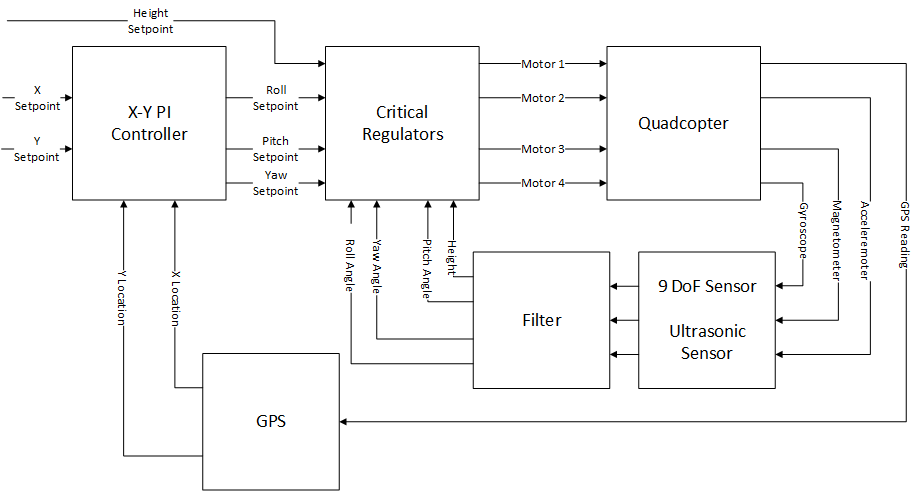
\includegraphics[width =0.7\paperwidth]{\DocRoot/images/Cascaded_Control}
	\caption{Block Diagram of Final control of the Quad-Rotor}
	\label{Fig: Block Diagram of Final control of the Quad-Rotor}
\end{figure}
The combination of gyroscopes and accelerometers are referred to as smart sensors, which estimates pitch, roll yaw and there respective rates.

The Kalman Filter and controller were designed and simulated using MatLab based on the quad-rotor model presented in \ref{eq: quad rotor model}. The current control set-points are roll,pitch and yaw, but the control has been developed for $x$ and $y$ to be made the set-points of the system. The current state used in the quad-rotor control scheme are as follows [$\gls{pitch},\gls{roll},\gls{yaw},\dot{\gls{pitch}},\dot{\gls{roll}},\dot{\gls{yaw}},h,\dot{h},\Delta\omega$]

\newpage
{
	\begin{description}[itemsep=1mm]
		\item[{\bf Where:-}]
		\item[\gls{pitch},\gls{roll},\gls{yaw}:] are the angle at which the quad-rotor is with respect to the $x,y$ and $z$ respectively.
		\item[$\dot{\gls{pitch}},\dot{\gls{roll}},\dot{\gls{yaw}}$:] are the rate of change of these angles
		\item[$h,\dot{h}$:] is the height and rate of change of height of the quad-rotor 
		\item[$\Delta\omega$:] is the differential thrust difference between the two opposing motors
		along an axis. 
	\end{description}
}

The type of controller designed to control the quad-rotor is an optimal controller, which controls the quad-rotor by selecting regulator gains for the best possible performance. To achieve this, the aspects of the plants behavior that are desired to be controlled must be incorporated in a mathematical expression referred to as the \enquote{cost function}. 

\section{Design of a \gls{lqr} Controller}
As the control scheme used on the quad-rotor was digital then any optimal controller used to stabilize the system had to be in discrete form too.Hence, the cost function to be minimized was of the discrete form and is defined as follows:- 

 \begin{equation}
 J_N  = \frac{1}{2} \sum_{n=0}^{N-1}(x_n^\intercal {\bf Q} x_n + u_n^\intercal {\bf R }u_n) + \frac{1}{2}x_N^\intercal {\bf Q}_N x_N
 \label{eq: discreter lqr}
 \end{equation}
 where $x$ and $u$ denote the states and inputs of the system respectively and {\bf Q} and {\bf R} are matrices chosen to apply the desired weights to various states and inputs respectively. 
 
 A controller designed by this approach is known as a \gls{dlqr} and is tuned by changing the ${\bf Q}$ and ${\bf R}$ matrices shown in \eqref{eq: discreter lqr} to give the optimal response. The ${\bf Q}$ and ${\bf R}$ matrices set a weighting on the state variable tracking and the control action respectively. If {\bf Q} is increased then a penalty is introduced which limits the deviation of the states from their set-points. Following from this if the {\bf Q} matrix is increase so too is the feedback gains. In contrast, if the {\bf R} matrix is increased, then aggressive control responses are penalized, which leads to a reduction in the feedback terms. Even though an \gls{lqr} controller is an optimal controller there are limitations inherent in its design. The main failing of an \gls{lqr} based control scheme is the fact that its frequency response rolls of at 20 dB per decade \cite[pg 584-617]{Artofcontrol}. Since the \gls{lqr} controller has such a poor frequency response it is often used injunction with a optimal filter such as the Kalman Filter so as to alleviate this problem.
 
 \subsection{Tuning of the {\gls{lqr}} controller}
 When a \gls{lqr} based control scheme is implemented there is two methods of tuning the controller, one is to set the {\bf Q} and very {\bf R} until the desired response is achieved. This form of tuning is possible as the \gls{lqr} controller is derived in a similar manner to Kalman Filter. Hence, a tuning approach similar to that used to tune the Kalman Filter in Chapter \ref{chap: kalman implem} can also be used to tune the \gls{lqr} controller. 
 
 The second approach is to use Bryson's Rule \cite{franklin2006feedback}. Bryson's Rule works by setting a maximum acceptable value of each state and then penalizes them accordingly. Bryson's Rule is commonly denoted as follows:-      
 
 \begin{align}
 \begin{split}
 Q_{ii} &= \frac{1}{(z_i^{max})^2}~~~~~~~~~~~~~~  i\in 1,2,\ddddot{}l\\
 R_{ii} &= \frac{1}{(u_j^{max})^2}~~~~~~~~~~~~~~        j\in 1,2,\ddddot{}m
 \end{split}
 \end{align}
 
 {	
 	\begin{description}[itemsep=1mm]
 		\item[Where:-]
 		\item[$z_i^{max}$:] is the maximum acceptable value of the $i$ state of the system 
 		\item[$u_i^{max}$:] is the maximum acceptable value of the $i$ input of the system.
 	\end{description}
 }
 
 which means the \gls{lqr} equation can be redefined as follows:-
 \begin{equation}
 J_N = \int_{0}^{\infty}\left(\sum_{i=1}^{l}Q_{ii}z_i(t)^2 + \sum_{j=1}^{m}R_{jj}u_{j}(t)^2\right)
 \end{equation}
 This method of tuning the \gls{lqr} controller was advantages as it allowed a limited to be set on states which in real life had limits and could saturate. An example of such a saturation is the angular velocity of the motors and the \gls{pwm} signal which also has an upper limit.  


\newpage
\subsection{Observer Design}
As the state space controller used on the quad-rotor required unmeasurable states, an observer is required to estimate these unknown states. An observer was designed which used sensor readings and the mathematical model of the quad-rotor presented in Section \ref{sec: quad-model} to estimate the unknown states.The observer required knowledge of the desired responses, which is achieved by the placement if its poles. A common method of designing an observer is by means of the Butterworth Constellation Technique, such an observer can easily be designed in MatLab by means of the \textit{place} function.

\subsubsection{Butherworth Constellation Technique}

\begin{figure}[h]
	\centering
	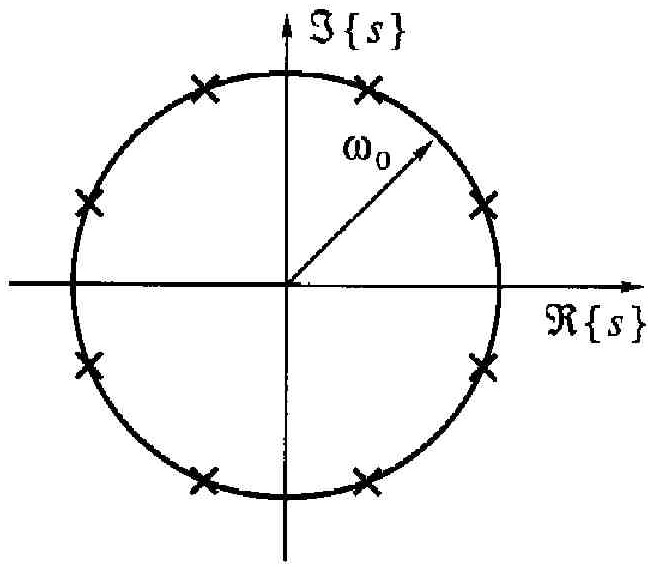
\includegraphics[width =0.4 \paperwidth]{\DocRoot/images/Butterworth_poles_2}
	\caption{8 Order Butterworth pole placement diagram }
	\label{Fig:butterworth diagram}
\end{figure}

Figure \ref{Fig:butterworth diagram} gives a graphical representation of the placing poles using the Butterworth Technique. The radius of the circle is $\omega_n$, found using the following:-

\begin{equation}
\frac{4}{\zeta \omega_n} = T_{s_{2\%}} \label{eq: observer design equation}
\end{equation}

 {	
 	\begin{description}[itemsep=1mm]
 		\item[Where:-]
 		\item[$\zeta$:] is the maximum acceptable value of the $i$ state of the system 
 		\item[$T_{s_2\%}$:] is the settling time of the observer.
 	\end{description}
 }

Once the observer was designed it was tested with the \gls{lqr} controller which was designed by means of \eqref{eq: discreter lqr}. The combination of the \gls{lqr} controller, observer and Kalman Filter the following response presented in Figure \ref{Fig:lqr controller}. Under this controller it was possible to control the roll,pitch and yaw axes.


\begin{figure}[h]
	\centering
	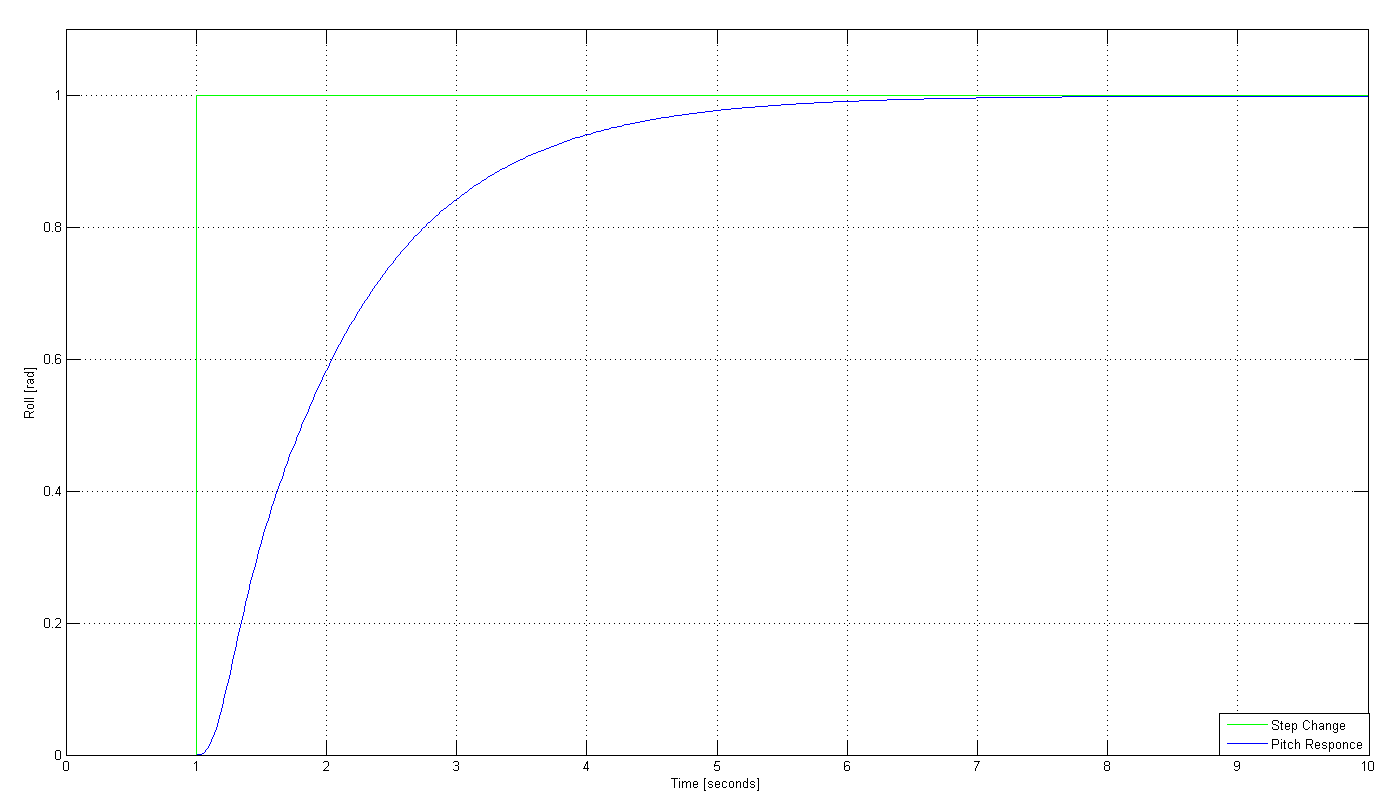
\includegraphics[width =0.6 \paperwidth]{\DocRoot/images/Roll_LQR1}
	\caption{Step response of the quad-rotor for the roll axis}
	\label{Fig:lqr controller}
\end{figure}
